\chapter{Картина мира субъекта деятельности} \label{chapt:review}

\section{Психологические предпосылки к созданию модели картины мира} \label{sect:psycho}

\subsection{Культурно"--~исторический подход Выготского}

Одна из первых успешных попыток формулировки общих принципов работы высших психических функций человека была предпринята отечественным психологом Л.\,С. Выготским в 20--30 гг. XX в. \cite{Vygotsky2005} и далее развивалась последователями его школы А.\,Н. Леонтьевым, А.\,Р. Лурия, П.\,Я. Гальпериным, П.\,И. Зинченко \cite{Zinchenko1959,Luria1963,Luria1970}. 

Культурно"--~исторический подход Выготского предлагает рассматривать в качестве основного фактора, который определяет формирование психических функций человека, социальную среду. Развитие мышления, формирование высших психических функций происходит не само по себе, а только путём использования человеком так называемых <<психологических орудий>>. Одним из основных таких орудий является любая система знаков, например, язык, письмо, системы счёта.

Такие психические функции как память, восприятие, мышление в своём развитии проходят через этап внешней деятельности, когда культурные средства, <<психологические орудия>> имеют предметный вид и соотносятся с какой-то определённой последовательностью действий. И только затем такая последовательность действий сворачивается, \textit{интериоризуется}, переходит из внешнего плана во внутренний. 

Такая автоматизация отрабатываемых действий наблюдается в поведении человека повсеместно. Можно считать, что первым установленным свойством картины мира было свойство интериориизации некоторой последовательности действий. Трансформация её с более высокого, энергозатратного, требующего больше времени на реализацию уровня на более низкий, быстрый и автоматизированный.

По Выготскому одной из функций картины мира в дополнение к интериоризации является также и процесс \textit{экстериоризации} некоторой автоматизированной последовательности действий в случае возникновения каких-либо препятствий для её обычного, быстрого выполнения. Интериоризация не является, таким образом, необратимой "--- структуры и процедуры её реализующие при необходимости могут быть выполнены в обратном порядке.

На этапе интериоризации человек развивается в культурном, психическом плане только постоянно участвуя в деятельности с другими членами коллектива. При этом все те действия, которые пока за него выполняют другие члены коллектива составляют так называемую <<зону ближайшего развития>>. Именно действия из этой зоны будут интериоризованы в первую очередь.

Любое развитие, в том числе и картины мира, по Выготскому это не постепенный ровный процесс, а стадиальный, когда периоды достаточно медленного накопления знаний и новых возможностей, сменяются короткими этапами кризиса. За время течения кризиса происходят качественные изменения структуры некоторых частей картины мира и протекающих в них процессов, влекущие за собой перестройку других частей и процессов и т.\,д. Запускается лавинный процесс, который достаточно быстро заканчивается и сменяется новым периодом медленного накопления. Ступенчатый характер процессов обновления картины мира можно считать вторым установленным её свойством.

Выготский был одним из первых психологов, который указал на роль знака и коллектива в функционировании картины мира субъекта. Выготский первым дал психологическую интерпретацию знака и чётко обозначил ту роль, которую знаки играют в развитии субъекта. Однако работа интериоризованных процессов и их связь с внешними знаками осталась за скобками.

\subsection{Теория деятельности Леонтьева}

Развитием и применением идей культурно"--~исторического подхода занимались многие последователи Выготского, среди которых огромную роль в формировании целостной психологической модели картины мира субъекта сыграл А.\,Н. Леонтьев \cite{Leontiev1975}.

Леонтьев считается автором теории деятельности в психологии, основы которой были заложены в конце 20 гг. XX в. Любая деятельность с точки зрения Леонтьева является предметной, а любой предмет отражается, или \textit{опосредуется}, субъектом с помощью некоторого психического образования, которое, следуя Выготскому, стали называть \textit{знаком}. Носителем таких отражений, для которых дополнительно выполняется условие отделения от внутренних характеристик, в теории деятельности считается \textit{сознание}.

По Леонтьеву деятельность субъекта глубоко иерархична. На самом высшем уровне находятся различные виды деятельности, отличающиеся друг от друга той потребностью, которая направляет ту или иную деятельность. На следующем уровне иерархии располагаются сознательные, не автоматизированные действия, каждое из которых задаётся некоторой целью, представлением о результате своего выполнения. Действие может иметь различный операционный состав в зависимости от условий реализации, что составляет третий уровень иерархии. Наконец, на самом нижнем уровне лежат психофизиологические механизмы, которые реализуют ограничения, накладываемые на форму операций свойствами организма субъекта деятельности.

Такая четырёхуровневая схема деятельности по Леонтьеву выделяет среди психических отражений предметов реального мира четыре вида единиц: потребности, мотивы, цели и условия. Каждая потребность рано или поздно опредмечивается, формируя мотив, который и является направляющей силой любой деятельности. Мотив при этом может не осознаваться. Мотив формирует зону целей, для достижения которых в рамках текущей деятельности выбираются соответствующие действия. Наконец, форму реализации действий определяют те или иные предметные условия, задающие операции (Рисунок~\ref{fg:activity}).

\begin{figure}[h]
	\centering	
	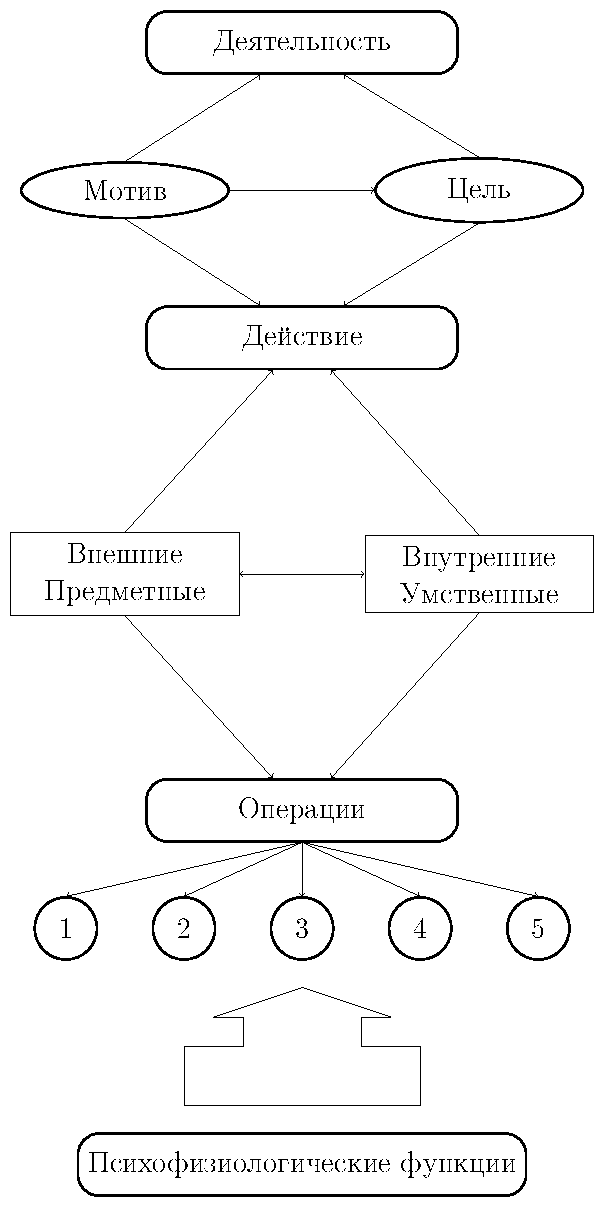
\includegraphics[width=0.3\linewidth]{psycho/activity}
	\caption{Структура деятельности по Леонтьеву.}
	\label{fg:activity}
\end{figure}

Для более подробного описания структуры деятельности Леонтьеву пришлось уточнить понятие знакового опосредования предметов, введённое Выготским. Были определены компоненты знака, отражающего некоторый реальный объект действительности. Первый компонент или образующая сознания "--- это чувственная ткань или образ, который является непосредственным, закодированным представлением предмета действительности в КМ. Второй компонент "--- это значение, которое Леонтьев определяет как преобразованную, свёрнутую в структуре языка идеальную форму существования предметного мира, его свойств, связей и отношений, раскрываемых совокупной общественной практикой. Система значений определяет общественно познанную реальность, поэтому изменение структуры значений происходит только как объективно"---историческое движение. Третий компонент знака, личностный смысл, или <<значение"--~для"--~меня>>, связывает имеющийся опыт субъекта, его потребности и свойства предметов действительности. Личностные смыслы всегда переживаются и задают эмоциональную окраску КМ субъекта.

Леонтьев стал основоположником общепринятой в настоящее время психологической модели картины мира. Он определил её основные образующие элементы и выделил различные уровни как процессов протекающих в самой картине мира, так и внешних действий, являющихся продуктами функционирования этой картины мира.

\subsection{Модель психики Артемьевой}

Понятие картины мира в современном представлении было дано в модели Е.\,Ю. Артемьевой \cite{Artemyeva1980}. Согласно её изложению в этой психической структуре следы взаимодействия с объектами фиксируются в системе опыта субъекта на семантическом уровне: <<мы смогли увидеть, как пристрастно отношение субъекта к входящему с ним в контакт предметному миру, как активно он (субъект) структурирует этот мир, создавая для себя его проекцию. Вещи всегда наделяются свойствами, характеризующими их взаимоотношения с субъектом. В частности, геометрические формы оказываются наделенными жестко сцепленными комплексами свойств, ведущими из которых являются эмоционально-оценочные свойства. У субъекта складывается картина мира, картина свойств вещей в их отношениях к нему и друг к другу>>. 

Артемьева изучала вопрос соотношения субъективного опыта и представления о мире или, в её терминологии, \textit{образа мира}, который несёт всю предысторию психической жизни субъекта. Чтобы объяснить процесс формирования представления о мире, Артемьева предположила существование некоторой структуры, являющейся регулятором и строительным материалом образа мира. Такая структура была разделена ею на три слоя. Первый слой, перцептивный мир, характеризуется существованием модальностей, соответствующих различным каналам восприятия внешнего мира. Второй слой, картина мира в узком смысле слова, представляет собой агрегацию различных семантик или систем амодальных значений. Третий слой, образ мира в узком смысле, содержит амодальные аффективные гипотезы, направляющие мыслительный процесс субъекта.

Глубокое исследование картины мира субъекта Артемьевой несмотря на разделение модели на три слоя и выделение более узкого определения картины мира, свидетельствует о продолжающемся углублении исследований различных компонент знака по Леонтьеву: образа (перцептивный мир), значения (семантический слой) и личностного смысла (аффективный слой), не меняя принципиально структуру модели.

\subsection{Зарубежные исследования КМ}

Одним из направлений зарубежных исследований в области построения психологических моделей картины мира является направление <<world view>>. Основные вопросы, на которые нацелены указанные исследования можно сформулировать следующим образом: 
\begin{itemize}
	\item Что такое мир, как он устроен и как он функционирует? 
	\item Почему человек чувствует то, что чувствует и как возникает у него определённое отношение к реальности? 
	\item Как человек действует в мире и как выбирает одну цель из множества возможных? 
	\item Как формируется субъективный образ мира?
\end{itemize}
 
Группа исследователей \cite{Aerts1994} в 1994 г. опубликовала программу проекта междисциплинарных работ, целью которого является создание модели <<world view>>, интегрирующей биологические, когнитивные, психологические, языковые, социологические, философские аспекты отношения к реальности. В качестве компонентов структуры <<world view>> выступают: онтология (модель существующего), объяснение (модель прошлого), предсказание (модель будущего), аксиология (теория ценностей), праксиология (теория деятельности) \cite{Aerts1994}. В \cite{Vidal2012} в <<world view>> были выделены объективная (<<концепция мира>>), субъективная (<<жизненный мир>>) и интерсубъективная (<<взгляды>>) составляющие. 

В психологическом плане <<world view>> может быть сопоставлен с концепциями <<философии жизни>> К.~Юнга, <<мировоззрения>> А.~Маслоу, <<гипотезы мира>> С.~Пеппера (S.\,C.~Pepper), <<возможных миров>> Дж.~Франка (J.\,D.~Frank), <<взгляда на реальность>> С.~Мессера (S.\,B.~Messer), <<системы конструктов Я-и-Мир>> Дж.~Коттлера (J.\,A.~Kottler) и Р.~Хецлера (R.\,J.~Hazler), <<ценностных ориентаций>>, <<неосознаваемых систем смыслов>>, <<неосознаваемых оснований выбора>>, <<ядерной культуры>> Ф.~Клюхона (F.\,R.~Kluckhohn) \cite{Koltko-Rivera2004}. 

\subsection{Выводы параграфа \ref{sect:psycho}}

На протяжении достаточно длительного периода психологических исследований картины мира субъекта деятельности были сформулированы следующие основные принципы её строения и функционирования:
\begin{itemize}
	\item существование двух уровней протекания психических процессов (внешний и внутренний план) и двух обратных процессов перехода процесса с одного уровня на другой: интериоризация (автоматизация) и экстериоризация (<<разворачивание>> в случае ошибок или затруднений);
	\item ступенчатый характер преобразования картины мира: медленные процессы накопления опыта сменяются быстрыми процессами реструктуризации;
	\item иерархичность процессов протекающих как внутри картины мира, так снаружи благодаря проявляющимся результатам её функционирования (схема деятельности субъекта);
	\item элементарной единицей картины мира является знак, опосредующий некоторое явление в окружающем мире, и состоящий из трёх компонент: образа, значения и личностного смысла.
\end{itemize}

\section{Нейрофизиологические исследования} \label{sect:neuro}

В последнее время исследования в области поиска нейрофизиологических коррелятов когнитивных функций вошли в список приоритетных направлений практически во всех развитых странах. В 2013~г. в США была анонсирована программа BRAIN INITIATIVE, а в 2014~г. под эгидой Департамента здравоохранения был запущен один из проектов данной программы под названием BRAIN \cite{NIH2014}. В 2013~г. в ЕС стартовал один из двух мегапроектов The Human Brain project (HBP, Проект моделирования мозга человека), объединяющий более 100 институтов из 24 стран \cite{HBP2014}. Оба эти проекта, как и многие менее крупные со схожей тематикой, имеют своей основной целью составление подробной карты участков головного мозга с указанием той когнитивной психической функции, за которую преимущественно отвечает та или иная область. Построение такой карты возможно только при наличии модели, которая бы на основе нейрофизиологических данных о строении головного мозга (как коры, так и подкорковых древних структур), предсказывала бы, какой вклад вносит определённая область в формирование интересующей функции. Подобные проекты базируются на огромном фактическом материале, накопленном за десятилетия проведения исследований строения мозга млекопитающих, и призваны заполнить пробел между сведениями о работе нейронов и их ансамблей и психологическими описаниями высших когнитивных функций. 

Поиск когнитивных коррелятов и описание общих нейрофизиологических оснований высших психических функций находится пока только в самом начале. Большинство тех работ в этой области, где проводится не только анализ фактического материала, но и приводится нейронная модель работы исследуемого процесса, ограничиваются попытками осветить только некоторые аспекты исследуемой функции. Примером могут служить многочисленные работы по моделям внимания, которые успешно объясняют и предсказывают только такие эффекты, как слепота к изменениям, ограниченность ресурса внимания, временные характеристики и т.\,п. \cite{Borji2013}.

\subsection{Состояние исследований на данный момент}

Попытки сформулировать базовые принципы, на основе которых необходимо проводить построение нейрофизиологических моделей предпринимались в ряде работ как в России (работы А.\,М.~Иваницкого \cite{Ivanitsky1996,IvanitskyE1996}), так и за рубежом (Д.\,М.~Эделмен (G.\,M.~Edelmen) \cite{Edelmen1981}) с 70~гг. XX~в. Так гипотеза повторного входа (или информационного синтеза) предполагает наличие некоторого замкнутого контура, состоящего из определённых участков и структур головного мозга (зрительная кора, ассоциативная кора, гиппокамп, гипоталамус, лобная кора). Прохождение сигнала по такому контуру активирует взаимосвязанные нейронные ансамбли, которые хранят информацию о значимости сигнала. Поступающие от них нервные импульсы возвращаются обратно в проекционную кору и накладываются на ещё сохраняющийся там след стимульного возбуждения. Только при успешном замыкании такого контура возникает ощущение и поступивший сигнал интерпретируется в контексте КМ субъекта (Рисунок~\ref{fg:ivanitsky_cyrcle}). 

\begin{figure}[h]
	\centering	
	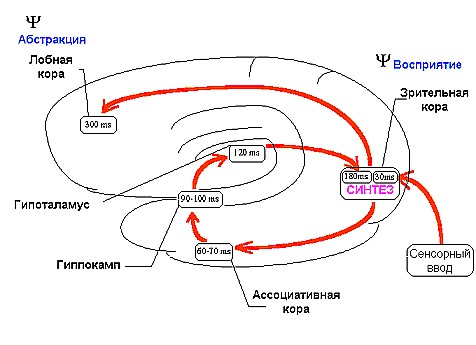
\includegraphics[width=0.7\linewidth]{phisio/ivanitsky_cyrcle.jpg}
	\caption{Круг ощущений по А.\,М.~Иваницкому (источник \cite{Ivanitsky1996}).}
	\label{fg:ivanitsky_cyrcle}
\end{figure}

Другой взгляд на базовые принципы организации моделей высших психических функций и картины мира субъекта содержится в так называемой теории рабочего пространства Б.\,Дж.~Баарса (B.\,J.~Baars) \cite{Baars2005}. В её нейронной реализации \cite{Dehaene2003} утверждается, что существует некоторое множество нейронов рабочего пространства, которые связаны с большим количеством автономных участков коры головного мозга. Эти участки коры, реализующие простые когнитивные функции, конкурируют за активацию нейронов рабочего пространства. Активация некоторого подмножества этих нейронов приводит к подавлению активации других таких нейронов и распространению самоподдерживающейся активности практически на всю кору. Таким образом, информация от захватившего глобальный ресурс когнитивного процесса становится доступной другим автономным процессам. Такая модель хорошо объясняет эффекты последовательности и избирательности высших психических функций, однако ничего не проясняет в механизмах их реализации. Подробнее см. подпараграф \ref{subsect:htm}.

Идея нейронов рабочего пространства схожа с описанием нейронов сознания известным отечественным нейрофизиологом Е.\,Н.~Соколовым \cite{Sokolov2004}. Соколов вводит понятие гештальт"--~пирамид, состоящих из нейронов-детекторов отдельных признаков. Вершиной такой пирамиды служит нейрон, гештальт"--~детектор, представляющий некоторый сложный объект в картине мира субъекта.

Среди последних работ на тему базовых принципов можно выделить исследование Дж.~Хокинса (J.~Hawkins) \cite{Hawkins2009}, где высказывается идея о том, что работа коры головного мозга базируется на множестве шестислойных колонок нейронов, организованных в иерархию и выполняющих достаточно простой набор элементарных функций. К таким функциям относятся фильтрация за счёт подавления слабого сигнала и предсказание формы следующей порции сигнала, поступающего с нижних слоев иерархии. В описании модели используется множество марковских цепей, элементы которых представляют низкоуровневые признаки. Каждая марковская цепь служит для вычисления вероятности наличия высокоуровневого признака на текущий момент. Подтверждение наличия признака проводится за счёт вероятностного вывода (распространения свидетельств), аналогичного выводу в баейсовских сетях доверия. Построенная Хокинсом модель иерархической временной памяти (HTM, Hierarchical temporal memory) хорошо решала задачи по моделированию восприятия, была применена в некоторых работах по распознаванию \cite{Bolotova2011} и легла в основу нескольких коммерческих проектов (Grok, Sighthound и др. \cite{NUM2014}). Несмотря на свою высокую перспективность, попыток дальнейшего развития модели для построения описания более сложных функций на данный момент предпринято не было.

Идея иерархической организации большого количества одинаковых достаточно простых базовых элементов используется практически во всех попытках построить нейрофизиологические модели когнитивных функций. Из отечественных работ здесь можно отметить исследования В.\,Я.~Сергина \cite{Sergin2008,Sergin2009,Sergin2011}, в которых вводится концепция объемлющих характеристик. Концептуальная модель Сергина предполагает наличие обратных связей в небольшом участке коры головного мозга, замкнутых на ту же область. Их наличие обеспечивает механизм процесса автоотождествления, который постулируется как основа всех когнитивных функций. Временные характеристики образующихся циклов на разных уровнях иерархии хорошо согласуются с экспериментом и могут объяснить некоторые психические феномены, однако математической модели в работах автора представлено не было.

Иерархия нейроподобных элементов встречается и в некоторых других отечественных работах. Так в \cite{Vartanov2011,Chernavsky2012} делается попытка построить иерархию элементов, которые бы могли кодировать поступающие сигналы в некоторые семантические структуры с использованием обратных связей и <<внутренних экранов>>. В этих работах используются те же идеи повторного входа, однако, реальных экспериментов, моделирующих хотя бы простейшие когнитивные функции, представлено пока не было.

\subsection{Теория глобального рабочего пространства}

Одной из основных теорий, которая предлагает объяснение некоторым особенностям работы высших когнитивных функций и которая на данный момент является самой распространённой в европейских работах, является теория Баарса \cite{Baars1988,Baars2005}.

Центральной идеей в теории глобального рабочего пространства (ГРП, Global workspace) Баарса является тот факт, что содержание высших психических функций доступно всем более низкоуровневым психическим процессам, таким как внимание, мышление, память и речь (Рисунок~\ref{fg:dehaene_gwt_a}). В связи с тем, что доступ к этому содержанию ограничен единственным потоком, теория ГРП естественным образом объясняет последовательную природу сознательного опыта.

Теория ГРП была изначально представлена в версии классной доски, когда отдельные, квази"--~независимые процессы сообщаются с центральным общедоступным ресурсом. Такая архитектура была впервые реализована в вычислительной модели взаимодействующих программных агентов С.~Франклина (S.~Franklin) и А.~Грессера (A.~Graesser) \cite{Franklin1999}.

\begin{figure}[h]
	\centering
	\begin{subfigure}[b]{0.3\textwidth}
		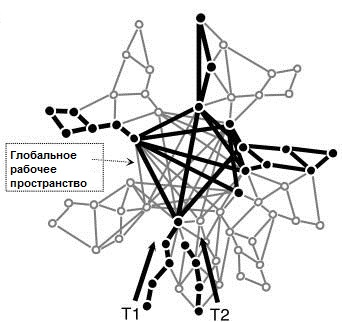
\includegraphics[width=\textwidth]{phisio/dehaene_gwt_a}
		\caption{}
		\label{fg:dehaene_gwt_a}
	\end{subfigure}
	~ 
	\begin{subfigure}[b]{0.3\textwidth}
		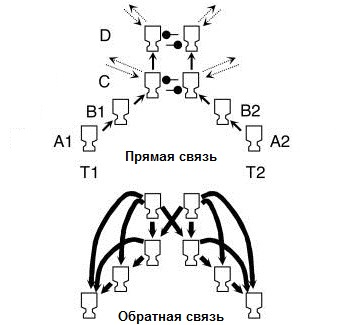
\includegraphics[width=\textwidth]{phisio/dehaene_gwt_b}
		\caption{}
		\label{fg:dehaene_gwt_b}
	\end{subfigure}
	~ 
	\begin{subfigure}[b]{0.3\textwidth}
		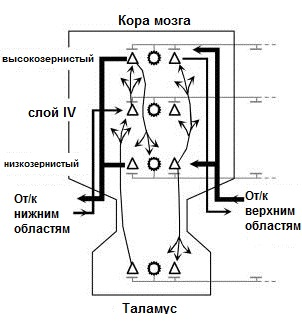
\includegraphics[width=\textwidth]{phisio/dehaene_gwt_c}
		\caption{}
		\label{fg:dehaene_gwt_c}
	\end{subfigure}
	\caption{Реализация теорий глобального рабочего пространства в работе Дехане (\cite{Dehaene2003}).}
	\label{fg:dehaene_gwt}
\end{figure}

С.~Дехане (S.~Dehaene) с коллегами \cite{Dehaene2003} предложили нейронную реализацию архитектуры глобального рабочего пространства, так называемое нейронное глобальное рабочее пространство (НГРП). Дехане, ссылаясь на нейрофизиологические данные о существовании стадии процесса восприятия с низкой пропускной способностью \cite{Chun1995}, постулирует общедоступность сигнала, поступающего с задних областей зрительной коры в НГРП и активирующего нейроны с длинными аксонами, распространяющими активность практически на всю кору. Возбуждённые нейроны подавляют активность остальных нейронов рабочего пространства, которые перестают обрабатывать поступающие сигналы. 

В своей модели Дехане с коллегами использовали простейшие спайковые нейроны, выдающие спонтанную активность при превышении уровня деполяризации мембраны некоторого порога. Эти нейроны организованы в простые трёхслойные колонки соединённые с сетью таламуса, через которую поступает входной сигнал (Рисунок~\ref{fg:dehaene_gwt}). Колонки в свою очередь связаны в иерархию, в которой присутствуют как близко действующие восходящие каналы распространения сенсорной информации, так и дальнодействующие нисходящие модулирующие связи, что согласуется с анатомическими и нейрофизиологическими данными \cite{Lamme2000,Felleman1991}. Первый тип связей реализуется с помощью AMPA"--~рецепторов, а второй "--- с помощью NMDA"--~рецепторов. Наиболее вероятен случай, когда глобальная активность обуславливается <<резонансом>> \cite{Llinas1998} между восходящей сенсорной информацией и нисходящим сигналом.

Для моделирования эффектов внимания (мигание внимания), была реализована простая четырёхуровневая иерархия, в которой конкурировали два типа сигналов $T_1$ и $T_2$ (Рисунок~\ref{fg:dehaene_gwt_b}), обрабатываемые невзаимодействующими параллельными перцептивными областям $A_i$ и $B_i$. По достижении сигналами $T_1$ и $T_2$ ассоциативных областей $C$ и $D$ начинается конкуренция между ними за активизацию соответствующих колонок рабочего пространства.

Модель порогового спайкого нейрона (зависимость напряжения на мембране нейрона $V$ от ёмкости мембраны $C_m$ и силы тока по времени) задавалась следующей формулой:

\begin{equation}
	\begin{split}
		C_mdV/dt=-g_{Leak}(V-V_{rest})-I_{NaP}-I_{KS}-I_{GABA}-I_{AMPA}-I_{NMDA}-\\
		-I_{SRA}-I_{input}-I_{neuromodul},
	\end{split}
\end{equation}
где $g_{Leak}$ означает ёмкость утечки, а $I_x$ "--- соответствующие веществам и типам нейромедиаторов $x$ токи, $I_{SRA}$ "--- ток адаптации в спайковой модели, $I_{input}$ "--- ток в момент подачи сигнала, $I_{neuromodul}$ "--- суммарные нейромодулирующие токи. Каждая таламо"--~кортикальная колонка была представлена 80 активными нейронам и 40 тормозными, схема связей между которыми представлена на Рисунок~\ref{fg:dehaene_gwt_c}.

Такая нейронная структура позволила Дехане с коллегами довольно успешно смоделировать известный психологический эффект мигания внимания \cite{Raymond1992}, который заключается во временном прерывании процесса восприятия сигналов с сохранением их обработки на нижних уровнях. Идея временного подавления активности небольшого количества нейронов глобального пространства достаточно просто объясняет этот эффект. Подбор временных характеристик порогового уравнения поляризаии мембраны нейрона позволяет достаточно точно повторить временные характеристики этого явления. Однако смещение акцентов на модель нейрона, а не на общие характеристики коры головного мозга является и основным препятствием для построения моделей более сложных эффектов и процессов в рамках этого подхода.

\subsection{Иерархическая временная память}\label{subsect:htm}

Смещение акцентов на рассмотрение общих свойств строения коры головного мозга было предпринято в работах Дж.~Хокинса и Д.~Георга \cite{George2005,Hawkins2009}. Хокинс постулирует, что основным инструментом построения картины мира субъекта является кора головного мозга, которая имеет одинаковое колоночное строение во всех своих областях и использует пространственно"--~временную иерархию для хранения построенной модели действительности, так называемую временную иерархическую память (ИВП).

Хокинс предлагает моделировать работу неокортекса с помощью узлов, организованных в дерево и использующих один и тот же алгоритм обучения и вывода, за счёт которого происходит сохранение пространственных шаблонов и их последовательностей. Прямой выход каждого узла состоит из представления тех или иных активных в данный момент последовательностей. Пространственные шаблоны фиксируют совпадение во времени последовательностей дочерних узлов. Иерархия узлов организована таким образом, что узлы более высокого уровня хранят шаблоны, представляющие большие масштабы пространства и большие промежутки времени, чем узлы более низкого уровня.

Математическое описание ИВП дано Георгом в виде порождающей модели (Рисунок~\ref{fg:hawkins_htm}). Каждый узел $N^i$ ($i$ "--- индекс узла) иерархии содержит множество синхронных шаблонов $c_1^i, c_2^i,\dots,c_{|C|}^i$ и множество марковских цепей $g_1^i,g_2^i,\dots,g_{|G|}^i$, где $|C|$ "--- общее количество шаблонов в узле, $|G|$ "--- общее количество марковских цепей в узле. Каждая марковская цепь $g_k^i$ определена на подмножестве множества синхронных шаблонов этого узла. Например, марковская цепь $g_1^{1,1}$ узла $N^{1,1}$ состоит из $4$ синхронных шаблонов: $c_1^{1,1}$, $c_3^{1,1}$, $c_4^{1,1}$ и $c_7^{1,1}$. Синхронный шаблон $c_j^i$ узла представляет одновременно активированные марковские цепи дочерних узлов. Например, шаблон $c_1^{2,1}$ узла $N^{2,1}$ на Рисунок~\ref{fg:hawkins_htm} определяется двумя марковскими цепями $g_1^{1,1}$ и $g_2^{1,2}$ дочерних узлов $N^{1,1}$ и $N^{1,2}$ соответственно. Синхронный шаблон, который задаётся путём отбора марковской цепи в высокоуровневом узле, активирует свои составляющие марковские цепи низкоуровневых дочерних узлов. Для конкретных синхронного шаблона и марковской цепи, которая активна в высокоуровневом узле, задаются конкурирующие последовательности синхронных шаблонов путём отбора активированных марковских цепей дочерних узлов.

\begin{figure}[h]
	\centering
	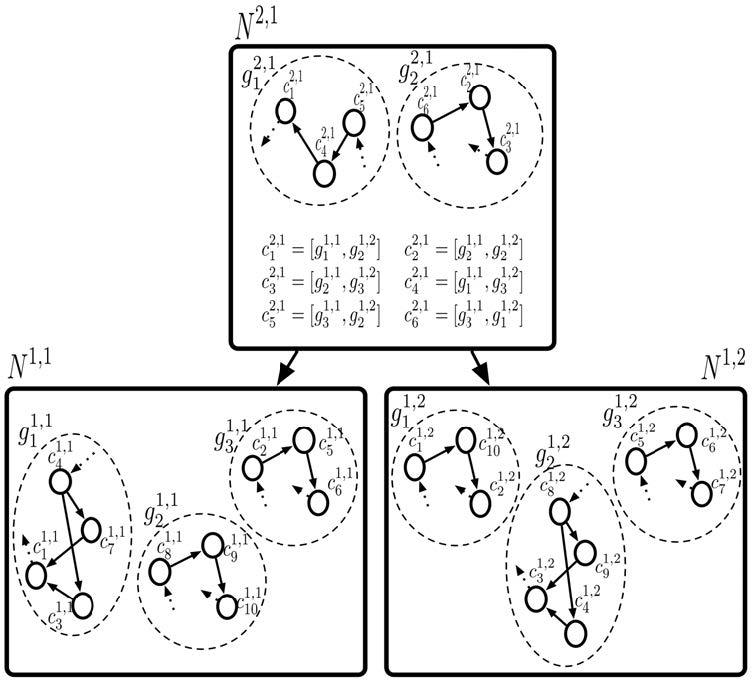
\includegraphics[width=0.7\linewidth]{mpf/hawkins_htm.jpg}
	\caption{Порождающая модель ИВП. Приведена простая двухуровневая порождающая модель ИВП, состоящая из трёх узлов (\cite{Hawkins2009}).}
	\label{fg:hawkins_htm}
\end{figure}

Процесс обучения ИВП на пространственно"--~временных данных представляет собой процесс построения синхронных шаблонов и марковских цепей в каждом узле на каждом уровне иерархии. Базовый алгоритм обучения состоит из двух операций:
\begin{itemize}
	\item сохранение некоторого фиксированного количества случайно выбранных генерируемых синхронных шаблонов,
	\item построение набора марковских цепей на множестве синхронных шаблонов путём обучения достаточно большой матрицы переходов.
\end{itemize}
В дальнейшем примере будет рассматриваться только тот случай, когда в один и тот же момент времени активен только один шаблон, хотя в работе авторов были реализованы и тот случай, когда активировалось определённое разреженное количество шаблонов.

Механизм вывода в сети ИВП основывается на распространении нового факта из одного узла сети вверх на все остальные. Распространение нового факта приводит к обновлению состояний узлов. Информация также распространяется и вниз по иерархии, обеспечивая механизмы внимания, сегментации и заполнения пропущенных фрагментов. В качестве алгоритма, реализующего вывод, Хокинсом был выбран алгоритм байесовского распространения степени уверенности.

В общем случае, сигнал, пришедший в узел ИВП с нижнего уровня, представляет функцию доверия на множестве дочерних марковских цепей. Данный узел преобразует этот сигнал в собственную функцию доверия на множестве своих синхронных шаблонов. Основываясь на истории полученных ранее сигналов, он вычисляет уровень доверия для каждой своей марковской цепи. Формируемый таким образом сигнал передаётся далее вверх по иерархии. В обратном направлении узел получает от родительских узлов функцию доверия на множестве своих марковских цепей. Далее марковские цепи шаг за шагом <<разворачиваются>> с целью вычисления нисходящего распределения вероятности на множестве синхронных шаблонов. Исходя из этого вычисляется функция уровня доверия узла на множестве дочерних марковских цепей. Формируемый таким образом сигнал передаётся дочерним узлам.

\begin{figure}[h]
	\centering
	\begin{subfigure}[b]{0.45\textwidth}
		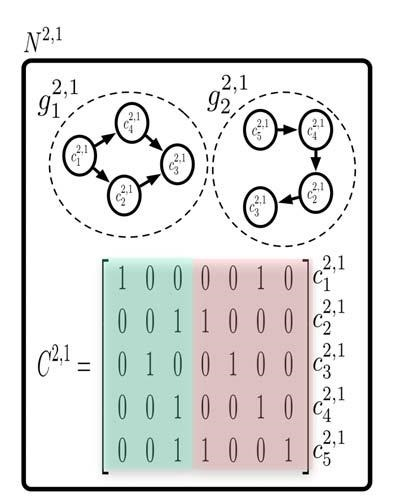
\includegraphics[width=\textwidth]{mpf/hawkins_htm_ex_a}
		\caption{}
		\label{fg:hawkins_htm_ex_a}
	\end{subfigure}
	~
	\begin{subfigure}[b]{0.45\textwidth}
		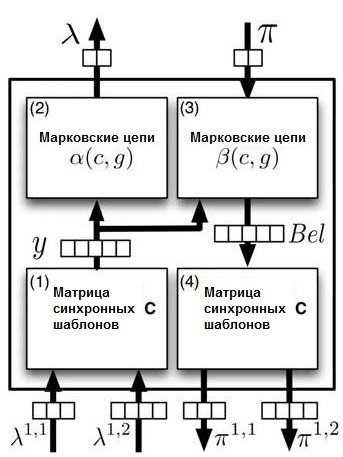
\includegraphics[width=\textwidth]{mpf/hawkins_htm_ex_b}
		\caption{}
		\label{fg:hawkins_htm_ex_b}
	\end{subfigure}
	\caption{Структура узла ИВП, входные и выходные данные узла (\cite{Hawkins2009}).}
	\label{fg:hawkins_htm_ex}
\end{figure}

В качестве примера в работе авторов приводится узел, содержащий 5 синхронных шаблонов и 2 марковские цепи (Рисунок~\ref{fg:hawkins_htm_ex_a}). Вероятностная матрица переходов марковской цепи $g_r$ обозначается как $P(c_i(t)|c_j(t-1),g_r)$. Как было сказано ранее, каждый узел получает на вход сигнал от дочерних узлов ($\lambda^{child\ index}$) и отправляет сигналы родительским узлам ($\lambda$). В обратном направлении, узел получает сигналы от родительских узлов ($\pi$) и отправляет обратные сигналы дочерним узлам ($\pi^{child\ index}$) (Рисунок~\ref{fg:hawkins_htm_ex_b}). Поступивший в момент времени $t$ с нижнего ровня факт обозначается ${}^-e_t$, а с верхних уровней "--- ${}^+e_t$.

Итоговая восходящая вероятность синхронного шаблона $c_i$ в момент времени $t$ вычисляется как произведение тех частей сообщения, которые соответствуют этому шаблону:
\begin{equation}
	y_t(i)=P({}^-e_t|c_i(t))\varpropto\prod_{j=1}^{M}\lambda_t^{m_j}(r_i^{m_j}),
\end{equation}
где $r_i^{m_j}$ обозначает номер марковской цепи $j$-го дочернего узла. Восходящая вероятность марковской цепи $g_r$ в момент времени $t$ вычисляется через специальную переменную состояния $\alpha$:
\begin{equation}
	\begin{split}
	\lambda_t(g_r)=P({}^-e_0^t|g_r(t)) = \sum_{c_t(t)\in C^k}\alpha_t(c_i, g_r),\\
	a_t(c_i,g_r )=P({}^-e_t|c_i(t))\sum_{c_i(t-1)\in C^k}P(c_i(t)|c_j(t-1),g_r)\alpha_{t-1}(c_j,g_r),\\
	\alpha_0(c_i,g_r)=P({}^-e_0|c_i(t=0))P(c_i(t=0)|g_r),
	\end{split}
\end{equation}
где символом ${}^-e_0^t$ обозначена последовательность входных сигналов с момента времени $0$ по момент времени $t$. Последовательность вычисления $\alpha$ представляет из себя процесс обновления переменной динамического программирования.

Степень уверенность для синхронного шаблона $c_i$ вычисляется с помощью сообщений от родительских узлов и с использованием переменной состояния $\beta$:

\begin{equation}
	\begin{split}
		Bel_t(c_i)\varpropto\sum_{g_r\in G^k}\beta_t(c_i,g_r),\\
		\beta_t(c_i,g_r)=P({}^-e_t|c_i(t))\sum_{c_j(t-1)\in C^k}P(c_i(t)|c_j(t-1),g_r)\beta_{t-1}(c_j,g_r),\\
		\beta_0(c_i,g_r)=P({}^-e_0|c_i(t=0))P(c_i|g_r)\pi_0(g_r).
	\end{split}
\end{equation}
В свою очередь, посылаемый дочерним узлам сигнал вычисляется как
\begin{equation}
	\pi^{m_j}(g_r)\varpropto\sum_i I(c_i)Bel(c_i),
\end{equation}
где
\begin{equation}
	I(c_i)=
	\begin{cases}
		1, & \text{если $g_r^{m_i}$ "--- часть шаблона $c_i$,}\\
		0, & \text{в противном случае.}
	\end{cases}
\end{equation}

В~модели Георга собраны практически все существенные для построения картины мира принципы, однако математическое описание с использованием марковских цепей оказывается слишком громоздким, чтобы можно было изучать какие-либо математические свойства узлов и их иерархий. Идея с матричным представлением, которая и используется в программной реализации ИВП, выглядит более перспективной.

\subsection{Выводы параграфа \ref{sect:neuro}}

В большом количестве работ нейрофизиологов, посвящённых построению нейронных моделей тех или иных психических процессов, выделяются следующие основные свойства <<физиологической реализации>> КМ:
\begin{itemize}
	\item существуют ансамбли нейронов одинаковой структуры, являющиеся элементарными ячейками для описания процессов, протекающих в коре головного мозга (колонки неокортекса),
	\item колонки организованы в иерархию, обладающую обратными связями,
	\item колонки хранят в себе пространственно"--~временные шаблоны, нарабатываемые с течением времени.
\end{itemize}

\section{Прикладная семиотика} \label{sect:semio}

Среди многих исследований, заложивших основы построения моделей картин мира, следует отметить отечественное направление в искусственном интеллекте появившееся в конце 90~гг. XX~в. благодаря работам Д.\,А.~Поспелова, А.\,М.~Мейстеля, Г.\,С.~Осипова и др. \cite{Osipov1995,Pospelov1996,Ehrlich1997,Osipov1999,Osipov2000b,Osipov2002a,Osipov2002b}. Данное направление получило название прикладная семиотика и уходило корнями в первые семиотические модели конца 60~гг. \cite{Pospelov1976}. Основная идея этого направления заключалась в использовании знакового описания когнитивных процессов, картины мира, для построения интеллектуальных систем представления знаний. Знак при этом определялся как исходный элемент любой семиотической системы и включал в себя три аспекта:
\begin{itemize}
	\item имя знака или синтаксический аспект знака,
	\item содержание знака или семантический аспект знака,
	\item назначение знака или прагматический аспект знака.
\end{itemize}

Данное определение хорошо реализуется в виде фреймовой структуры, в которой имя фрейма соответствует имени знака, имена обычных слотов, связанные с ними ограничения, условия, области определения значений "--- содержанию знака, а слоты, содержащие в качестве значений имена присоединённых процедур "--- назначению знака \cite{Osipov1999}. 

Одной из основных задач, формулируемых в прикладной семиотике была задача изучения природы и свойств отношений моделирования, которые возникают между системой знаков и той областью реального мира, которая с помощью неё описывается. Объектами изучения прикладной семиотики являются не знаки и знаковые системы сами по себе, а  их применение в системах представления знаний при решении различных практических задач.

Введение понятия семиотической системы, в которой состояния соответствуют фиксированным формальным системам, а смена состояний определяется изменением договорённостей об аспектах знака, позволяет моделировать процессы, протекающие в открытых, динамических системах. При этом под сменой состояния подразумевается изменение параметров формальной системы: аксиом, правил вывода, стратегий поиска решений и т.\,д. Всё вышесказанное формализуется следующим определением \cite{Osipov2002a}.

\begin{Def}
	Семиотической системой $W$ называется упорядоченная восьмёрка множеств:
	\begin{equation}
		W=<T,R,A,P,\tau,\rho,\alpha,\pi>,
	\end{equation} 
	где	$T$ "--- множество основных символов, $R$ "--- множество синтаксических правил, $A$ "--- множество знаний о предметной области, $P$ "--- множество правил вывода решений (прагматических правил), $\tau$ "--- правила изменения множества $T$, $\rho$ "--- правила изменения множества $R$, $\alpha$ "--- правила изменения множества $A$, $\pi$ "--- правила изменения множества $P$.
\end{Def}

Именно в семиотике, в том числе прикладной, были сформулированы первые схемы образования нового знака. Приведём такую схему в случае моделирования знака с помощью треугольника Фреге (Рисунок~\ref{fg:frege_sign}) \cite{Frege2000,Pirs2000}. В реальном мире имеются такие сущность как объекты, процессы, все они называются денотатами. В результате отражения этих сущностей в сознании субъекта возникает представление о денотатах. При этом представление "--- это интегрированный образ (в психологии "--- гештальт), скрывает за собой денотат, делая его недоступным непосредственно.

\begin{figure}[h]
	\centering
	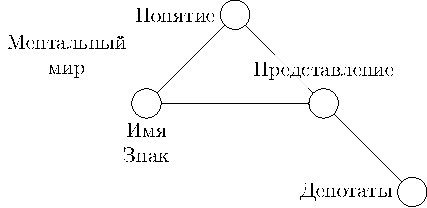
\includegraphics[width=0.7\linewidth]{signs/frege_tri}
	\caption{Треугольник Фреге.}
	\label{fg:frege_sign}
\end{figure}

Сталкиваясь с различными денотатами, человек накапливает определённую информацию о них. Некоторые из них он не различает, считая их проявлением одной и той же сущности, другие чем-то отличаются друг от друга. Для реализации такого различения и вводятся специфические имена, связанные с представлениями о том или ином виде сущности. На основе врождённой у человека процедуры выявления сходства"--~различия формируется и понятие о сущностях с данным именем.

Таким образом, наблюдение за единичным экземпляром сущности вызывает необходимость сформировать процедуру её узнавания, дать ей имя, а затем сформировать обобщённое представление об этой сущности (понятие). Со связями между именем, представлением и понятием ассоциированы процедуры, характерные для мышления человека.

Связь <<имя "--- понятие>> позволяет с одной стороны активизировать в памяти все сведения о свойствах данной сущности, а с другой, действуя в обратном направлении, позволяет по имплицитному описанию определить имя сущности. Связь <<представление "--- понятие>> позволяет по представлению сущности найти информацию о её свойствах и наоборот. Наконец, связь <<имя "--- представление>> необходима для соотнесения представления о денатате с его именем, примером работы которой могут служить алгоритмы распознавания образов.

В прикладной семиотике даётся и первое определение знака, позволяющее использовать его для построения моделей картины мира субъекта.

\begin{Def}
	Информационная единица, структурой которой является треугольник Фреге, где вершины отождествляются с именем, понятием и представлением, называется знаком.
\end{Def}

Компоненты знака могут иметь свою, достаточно сложную, структуру. Так, знак может содержать информацию о связях наследования, при этом множество знаков с отношениями наследования образуют иерархическую структуру. При этом типов отношений наследования может быть несколько: <<элемент "--- класс>>, <<часть "--- целое>>, <<вид "--- род>> "--- отличающихся тем, какие свойства наследуются. Таким образом, в прикладной семиотике впервые описываются отношения на множестве знаков и их свойства. Кроме отношения наследования в прикладной семиотике вводятся и горизонтальные типы отношений, например отношение <<причина "--- следствие>>. Система знаков с иерархическими и одноуровневыми отношениями называется \textit{семиотической сетью}, в которой каждая вершина может быть в свою очередь сетью.

Важным понятием, которое вводится в прикладной семиотике, является понятие активности сети знаков (по аналогии с понятием активности баз знаний С.\,К.~Дулина \cite{Dulin2005}). На семиотической сети специальными процедурами определяются те её участки, для которых имеется некоторое <<напряжение>>, т.\,е. существует диссонанс. При задании некоторой меры такой рассогласованности и при достижении её критического уровня, запускаются отдельные процедуры по устранению диссонанса. Для их активации вводится специальный тип знаков, \textit{метазнаки}, у которых денотатами служат определённые фрагменты сети знаков. Формируется так называемый метауровень описания.

С введением метауровня треугольник Фреге превращается в более сложную структуру, называемую квадратом Поспелова \cite{Osipov2000b} (Рисунок~\ref{fg:pospelov_sq}). Первая вершина квадрата определяет синтаксис, или способ кодирования знака, вторая  "--- семантику, или понятие о знаке, третья соответствует прагматике "--- тем процедурам, которые связаны с этим знаком. Новая, четвёртая вершина соответствует фрагменту некоторой структуры на множестве знаков и играет роль денотата метазнака. Стороны квадрата и его диагональ соответствуют различным процедурам, связывающим компоненты знака. 

\begin{figure}[h]
	\centering
	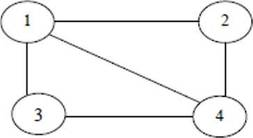
\includegraphics[width=0.5\linewidth]{signs/pospelov_sq}
	\caption{Квадрат Поспелова.}
	\label{fg:pospelov_sq}
\end{figure}
	
Наличие метауровня позволяет ввести внутреннюю интерпретируемость, а также снабжает знаковые системы свойством рефлексии, что является ключевым моментом на пути моделирования высших когнитивных функций, протекающих в картине мира субъекта деятельности.

%\newpage
%============================================================================================================================

\section{Выводы} \label{sect:concl}

Несмотря на большое количество имеющихся работ, в самых различных областях знаний, таких как психология, нейрофизиология, семиотика, искусственный интеллект, единого описания модели высших психических функций и процессов, протекающих в картине мира субъекта, выполнено не было. Однако были сформулированы базовые принципы, на которых должна строиться такая единая модель. К таким принципам и свойствам относятся: иерархичность как строения, так и протекающих в КМ процессов, активность КМ, существование элементарной единицы КМ, кодирование пространственно"--~временных шаблонов, наличие обратных связей. 

Из анализа проведённых исследований в данном направлении можно сделать вывод, что базовым элементом модели картины мира должен служить знак, строение которого на внешнем, синтаксическом уровне, задаётся в рамках психологических данных и теорий психических функций, а строение на внутреннем, семантическом уровне, согласуется с нейрофизиологическими данными о строении коры головного мозга человека.
%\newpage
%============================================================================================================================

\clearpage